% v2-acmtog-sample.tex, dated March 7 2012
% This is a sample file for ACM Transactions on Graphics
%
% Compilation using 'acmtog.cls' - version 1.2 (March 2012), Aptara Inc.
% (c) 2010 Association for Computing Machinery (ACM)
%
% Questions/Suggestions/Feedback should be addressed to => "acmtexsupport@aptaracorp.com".
% Users can also go through the FAQs available on the journal's submission webpage.
%
% Steps to compile: latex, bibtex, latex latex
%
% For tracking purposes => this is v1.2 - March 2012
\documentclass{acmtog} % V1.2

%\acmVolume{VV}
%\acmNumber{N}
%\acmYear{YYYY}
%\acmMonth{Month}
%\acmArticleNum{XXX}
%\acmdoi{10.1145/XXXXXXX.YYYYYYY}

\acmVolume{1}
\acmNumber{1}
\acmYear{2017}
\acmMonth{December}
\acmArticleNum{1}
\usepackage{float}
\usepackage{graphicx}
\usepackage{amsmath}
\usepackage{listings}
\usepackage{amssymb}


% Copyright
\setcopyright{rightsretained}


\begin{document}

\markboth{V. F. Pamplona et al.}{Photorealistic Models for Pupil Light Reflex and Iridal Pattern Deformation}

\title{Report of Chapter 11: Abstraction Methods } % title

\author{Qifeng Lin \\ 17214656}
% NOTE! Affiliations placed here should be for the institution where the
%       BULK of the research was done. If the author has gone to a new
%       institution, before publication, the (above) affiliation should NOT be changed.
%       The authors 'current' address may be given in the "Author's addresses:" block (below).
%       So for example, Mr. Fogarty, the bulk of the research was done at UIUC, and he is
%       currently affiliated with NASA.


\maketitle

\section{Review}
    \quad Abstraction Methods are used to verify a system by reducing a complex problem "$\mathcal{A}\models\phi$" to a much simpler problem "does $\mathcal{A}'\models\phi'$". If the size of the automaton is very large because of combinatorial explosion or if the model checker cannot handle automata using a given construction such as integer variables, then imposing abstraction methods is very useful to tackle these problems. In this chapter, three classical abstraction methods are introduced: abstraction by state merging, abstraction on the variables and abstraction by restriction.

    \subsection{Abstraction by merging states}
        \quad Abstraction by merging states can be showed as Fig 1.
        \begin{figure}[H]
          \centering
          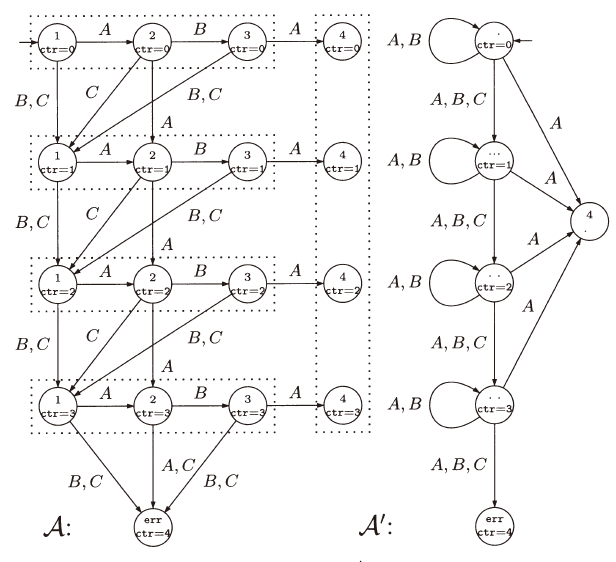
\includegraphics[width=3.0in, height=2.0in]{1.png}
          \caption{The digicode $\mathcal{A}$, and its variant $\mathcal{A}'$ after merging}
        \end{figure}
        It is obvious that the number of transitions has been reduced after merging. Then the abstract automaton can be used to verify the correctness, which is generally safety properties. The principle is explained based on following observations:
        \begin{enumerate}
          \item $\mathcal{A}'$ has more behaviors than $\mathcal{A}$. It is obvious that some extra behaviors are imported. For example, self loops occur in the variant $\mathcal{A}'$ while not occur in $\mathcal{A}$.
          \item The more behaviors an automaton has, the fewer safety properties it fulfills.
          \item Thus, if $\mathcal{A}'$ satisfies a safety property $\phi$ then a \textit{fortiori} $\mathcal{A}$ satisfies $\phi$. Suppose that if $\mathcal{A}'$ satisfies a safety property $\phi$ and if each execution of $\mathcal{A}$ is also an execution of $\mathcal{A}'$, then $\mathcal{A}$ also satisfy $\phi$. It is not hard to understand because each execution of $\mathcal{A}$ is also an execution of $\mathcal{A}'$.
          \item However, if $\mathcal{A}'$ does not satisfy $\phi$, no conclusions can be drawn about $\mathcal{A}$. This is also spoken as \textit{one-way preservation}. Suppose that $\phi$ does not hold in $\mathcal{A}'$, then some behaviors of $\mathcal{A}'$ are unsafe. But these behaviors may originate from the folding while not occur in $\mathcal{A}$. Actually, abstraction methods are often \textit{one-way}.
        \end{enumerate}

        After demonstrating observations on the abstract automaton, then explaining how to merge states is important. In principle, \textit{we must never merge states that are not labelled with the same properties}. But the restriction is too strong to apply. Thus, a weak restriction is proposed: \textit{if merging is used to check a given a property, then only the propositions occurring in $\phi$ are relevant}. It is divided into two cases: if a proposition $P$ only appears in positive form in $\phi$ or not. For the former, the resulting supper-state will carry the label $P$ if and only if all the merged carried it. For the latter, we may add propositions if these only occur negatively in $\phi$. But it is often hard to figure out if $P$ only occurs negatively and thus it will cause some error.

        Unfortunately, there is no tool to perform merging states automatically. Therefore, it is often completed by hand and thus may cause errors easily.

    \subsection{Abstraction on the Variables}
        \quad\textit{Abstraction on the variables} is used to deal with automata with variables. Under the condition, ignoring the variables or deleting the variables are often imported to perform abstraction. Take digicode as an example to state the procedures. The digicode before deleting variables is showed as Fig 2 and the one after deleting variables is showed as Fig 3, which is denoted as $\mathcal{A}$ and $\mathcal{A}'$ respectively.
        \begin{figure}[H]
          \centering
          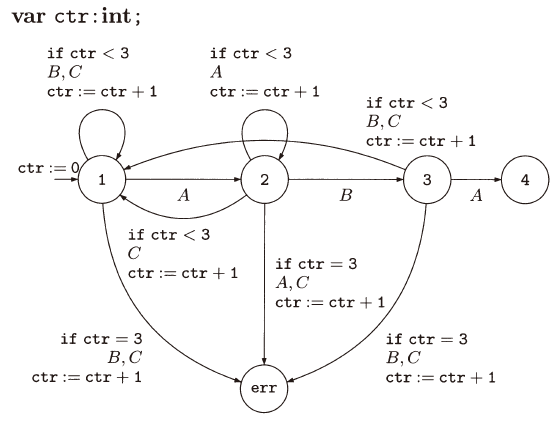
\includegraphics[width=3.0in, height=2.0in]{2.png}
          \caption{The digicode before unfolding}
        \end{figure}
        \begin{figure}[H]
          \centering
          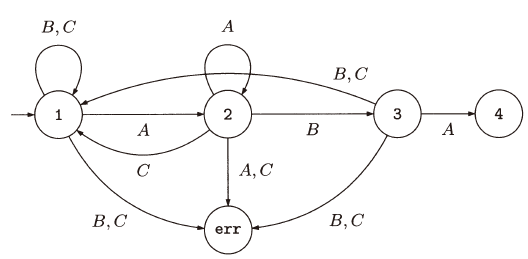
\includegraphics[width=3.0in, height=1.0in]{3.png}
          \caption{The digicode without the variables (nor the guards)}
        \end{figure}
        After deleting variables, it can be observed that $\mathcal{A}'$ inherits more behaviors than $\mathcal{A}$ and thus all the safety properties satisfied by $\mathcal{A}'$ are a \textit{fortiori} satisfied by $\mathcal{A}$. In this way, abstraction on the variables is similar to abstraction by merging states and it is easy to implement. But its main weakness it its coarseness for which the variables are necessary in most cases.

        There is a special case in abstraction on the variables: the variables are bounded variables. by bounding the domain of a variable v of an automaton $\mathcal{A}$, one can obtain an automaton $\mathcal{A}'$ whose behaviors is not totally different from that of $\mathcal{A}$. By appropriate modification of the guards, it is possible to guarantee that $\mathcal{A}'$ has more behaviors than $\mathcal{A}$ so that the satisfaction of safety properties can be transferred from $\mathcal{A}'$ to $\mathcal{A}$. Consider digicode again, by restricting the possible values of \textbf{ctr} to the interval 0..1 with the interpretation that these are values modulo 2, the result is showed as Fig 5.
        \begin{figure}[H]
          \centering
          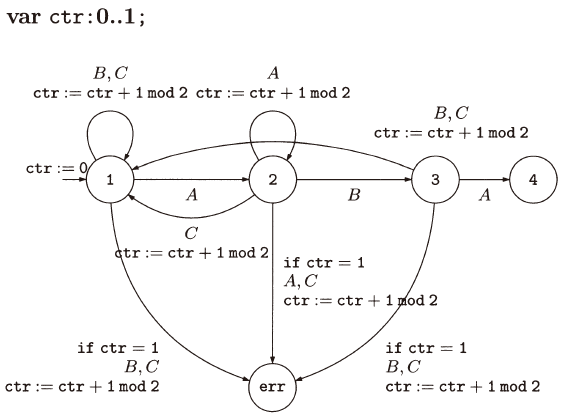
\includegraphics[width=3.0in, height=2.0in]{7.png}
          \caption{The digicode with a modulo 2 counter}
        \end{figure}
        
        It should be noticed that the guards if \textbf{ctr} = 3 , if \textbf{ctr} $<$ 3 and if \textbf{ctr} $\neq$ 3 haven been replaced by if \textbf{crt} = 1, \textbf{true} and \textbf{true} respectively. 
        
        After all, the principle which must constantly guide the user is the necessity to ensure that the simplifies system has more behaviors than the original system, so that the satisfaction of the variant can be transferred to the original one.
        

    \subsection{Abstraction by Restriction}
        \quad Restriction is a particular form of simplification that operates by forbidding some behaviors. Compared with previous abstraction by merging states and on the variables, if $\mathcal{A}'$ is obtained from $\mathcal{A}$ by restriction, then all the behaviors of $\mathcal{A}'$ are behaviors of $\mathcal{A}$. If $\mathcal{A}'$ does not satisfy a safety property , then a \textit{fortiori} neither does $\mathcal{A}$. Therefore, it is often used to prove that a safety property does not hold but not to prove the correctness of $\mathcal{A}$. The great advantage of restrictions is their simplicity, both conceptual and implementational.
        
        Observer automata is a kind of restriction method by restricting legitimate behaviors of a system to those accepted by an automaton outside the system, called \textit{observer automaton}. Consider digicode again, and the observer automaton is showed as Fig 5. The observer automaton states that desired property can be proved by only considering the behaviors in which a single $A$ may occur (the number of occurrences of $B$ and $C$ remains arbitrary).
        \begin{figure}[H]
          \centering
          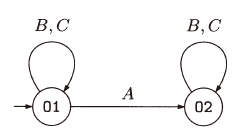
\includegraphics[width=1.5in, height=0.8in]{4.png}
          \caption{$\mathcal{O}$, an observer automaton for the digicode}
        \end{figure}
        
        The it is possible to synchronize the digicode and the observer $\mathcal{O}$. The result is depicted on Fig 6, which only keeps the reachable states and performs unfolding.
        \begin{figure}[H]
          \centering
          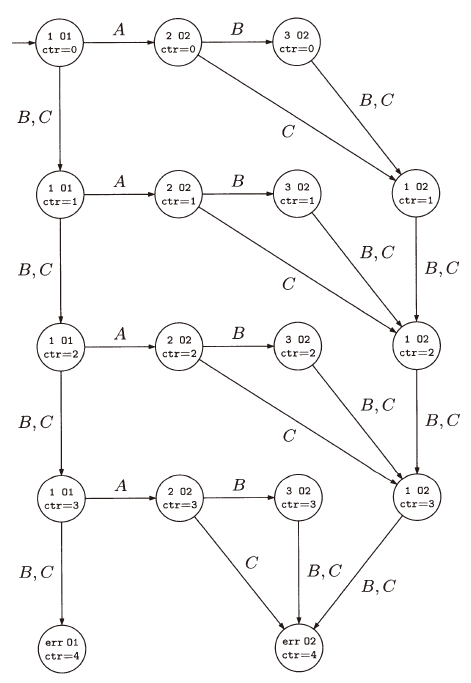
\includegraphics[width=3.0in, height=3.0in]{6.png}
          \caption{The synchronized digicode with its observer}
        \end{figure}
        
        Compared with the unfolding of the digicode in Fig 1, the number of paths has been reduced here although the number of states can increase because of the fact that the observer automaton adds a component. In this way, we can reduce behaviors and simplify the automaton. 
\section{Summary}
    \quad This chapter mainly introduces three classical abstraction methods:  abstraction by state merging, abstraction on the variables and abstraction by restriction, which is used to transform a complex problem "does $\mathcal{A}\models\phi$" to a simple problem "$\mathcal{A}'\models\phi'$". They all have their advantages and disadvantage. But they are all useful to perform simplification.



\end{document}
% End of v2-acmtog-sample.tex (March 2012) - Gerry Murray, ACM
